
% Default to the notebook output style

    


% Inherit from the specified cell style.




    
\documentclass[11pt]{article}

    
    
    \usepackage[T1]{fontenc}
    % Nicer default font (+ math font) than Computer Modern for most use cases
    \usepackage{mathpazo}

    % Basic figure setup, for now with no caption control since it's done
    % automatically by Pandoc (which extracts ![](path) syntax from Markdown).
    \usepackage{graphicx}
    % We will generate all images so they have a width \maxwidth. This means
    % that they will get their normal width if they fit onto the page, but
    % are scaled down if they would overflow the margins.
    \makeatletter
    \def\maxwidth{\ifdim\Gin@nat@width>\linewidth\linewidth
    \else\Gin@nat@width\fi}
    \makeatother
    \let\Oldincludegraphics\includegraphics
    % Set max figure width to be 80% of text width, for now hardcoded.
    \renewcommand{\includegraphics}[1]{\Oldincludegraphics[width=.8\maxwidth]{#1}}
    % Ensure that by default, figures have no caption (until we provide a
    % proper Figure object with a Caption API and a way to capture that
    % in the conversion process - todo).
    \usepackage{caption}
    \DeclareCaptionLabelFormat{nolabel}{}
    \captionsetup{labelformat=nolabel}

    \usepackage{adjustbox} % Used to constrain images to a maximum size 
    \usepackage{xcolor} % Allow colors to be defined
    \usepackage{enumerate} % Needed for markdown enumerations to work
    \usepackage{geometry} % Used to adjust the document margins
    \usepackage{amsmath} % Equations
    \usepackage{amssymb} % Equations
    \usepackage{textcomp} % defines textquotesingle
    % Hack from http://tex.stackexchange.com/a/47451/13684:
    \AtBeginDocument{%
        \def\PYZsq{\textquotesingle}% Upright quotes in Pygmentized code
    }
    \usepackage{upquote} % Upright quotes for verbatim code
    \usepackage{eurosym} % defines \euro
    \usepackage[mathletters]{ucs} % Extended unicode (utf-8) support
    \usepackage[utf8x]{inputenc} % Allow utf-8 characters in the tex document
    \usepackage{fancyvrb} % verbatim replacement that allows latex
    \usepackage{grffile} % extends the file name processing of package graphics 
                         % to support a larger range 
    % The hyperref package gives us a pdf with properly built
    % internal navigation ('pdf bookmarks' for the table of contents,
    % internal cross-reference links, web links for URLs, etc.)
    \usepackage{hyperref}
    \usepackage{longtable} % longtable support required by pandoc >1.10
    \usepackage{booktabs}  % table support for pandoc > 1.12.2
    \usepackage[inline]{enumitem} % IRkernel/repr support (it uses the enumerate* environment)
    \usepackage[normalem]{ulem} % ulem is needed to support strikethroughs (\sout)
                                % normalem makes italics be italics, not underlines
    

    
    
    % Colors for the hyperref package
    \definecolor{urlcolor}{rgb}{0,.145,.698}
    \definecolor{linkcolor}{rgb}{.71,0.21,0.01}
    \definecolor{citecolor}{rgb}{.12,.54,.11}

    % ANSI colors
    \definecolor{ansi-black}{HTML}{3E424D}
    \definecolor{ansi-black-intense}{HTML}{282C36}
    \definecolor{ansi-red}{HTML}{E75C58}
    \definecolor{ansi-red-intense}{HTML}{B22B31}
    \definecolor{ansi-green}{HTML}{00A250}
    \definecolor{ansi-green-intense}{HTML}{007427}
    \definecolor{ansi-yellow}{HTML}{DDB62B}
    \definecolor{ansi-yellow-intense}{HTML}{B27D12}
    \definecolor{ansi-blue}{HTML}{208FFB}
    \definecolor{ansi-blue-intense}{HTML}{0065CA}
    \definecolor{ansi-magenta}{HTML}{D160C4}
    \definecolor{ansi-magenta-intense}{HTML}{A03196}
    \definecolor{ansi-cyan}{HTML}{60C6C8}
    \definecolor{ansi-cyan-intense}{HTML}{258F8F}
    \definecolor{ansi-white}{HTML}{C5C1B4}
    \definecolor{ansi-white-intense}{HTML}{A1A6B2}

    % commands and environments needed by pandoc snippets
    % extracted from the output of `pandoc -s`
    \providecommand{\tightlist}{%
      \setlength{\itemsep}{0pt}\setlength{\parskip}{0pt}}
    \DefineVerbatimEnvironment{Highlighting}{Verbatim}{commandchars=\\\{\}}
    % Add ',fontsize=\small' for more characters per line
    \newenvironment{Shaded}{}{}
    \newcommand{\KeywordTok}[1]{\textcolor[rgb]{0.00,0.44,0.13}{\textbf{{#1}}}}
    \newcommand{\DataTypeTok}[1]{\textcolor[rgb]{0.56,0.13,0.00}{{#1}}}
    \newcommand{\DecValTok}[1]{\textcolor[rgb]{0.25,0.63,0.44}{{#1}}}
    \newcommand{\BaseNTok}[1]{\textcolor[rgb]{0.25,0.63,0.44}{{#1}}}
    \newcommand{\FloatTok}[1]{\textcolor[rgb]{0.25,0.63,0.44}{{#1}}}
    \newcommand{\CharTok}[1]{\textcolor[rgb]{0.25,0.44,0.63}{{#1}}}
    \newcommand{\StringTok}[1]{\textcolor[rgb]{0.25,0.44,0.63}{{#1}}}
    \newcommand{\CommentTok}[1]{\textcolor[rgb]{0.38,0.63,0.69}{\textit{{#1}}}}
    \newcommand{\OtherTok}[1]{\textcolor[rgb]{0.00,0.44,0.13}{{#1}}}
    \newcommand{\AlertTok}[1]{\textcolor[rgb]{1.00,0.00,0.00}{\textbf{{#1}}}}
    \newcommand{\FunctionTok}[1]{\textcolor[rgb]{0.02,0.16,0.49}{{#1}}}
    \newcommand{\RegionMarkerTok}[1]{{#1}}
    \newcommand{\ErrorTok}[1]{\textcolor[rgb]{1.00,0.00,0.00}{\textbf{{#1}}}}
    \newcommand{\NormalTok}[1]{{#1}}
    
    % Additional commands for more recent versions of Pandoc
    \newcommand{\ConstantTok}[1]{\textcolor[rgb]{0.53,0.00,0.00}{{#1}}}
    \newcommand{\SpecialCharTok}[1]{\textcolor[rgb]{0.25,0.44,0.63}{{#1}}}
    \newcommand{\VerbatimStringTok}[1]{\textcolor[rgb]{0.25,0.44,0.63}{{#1}}}
    \newcommand{\SpecialStringTok}[1]{\textcolor[rgb]{0.73,0.40,0.53}{{#1}}}
    \newcommand{\ImportTok}[1]{{#1}}
    \newcommand{\DocumentationTok}[1]{\textcolor[rgb]{0.73,0.13,0.13}{\textit{{#1}}}}
    \newcommand{\AnnotationTok}[1]{\textcolor[rgb]{0.38,0.63,0.69}{\textbf{\textit{{#1}}}}}
    \newcommand{\CommentVarTok}[1]{\textcolor[rgb]{0.38,0.63,0.69}{\textbf{\textit{{#1}}}}}
    \newcommand{\VariableTok}[1]{\textcolor[rgb]{0.10,0.09,0.49}{{#1}}}
    \newcommand{\ControlFlowTok}[1]{\textcolor[rgb]{0.00,0.44,0.13}{\textbf{{#1}}}}
    \newcommand{\OperatorTok}[1]{\textcolor[rgb]{0.40,0.40,0.40}{{#1}}}
    \newcommand{\BuiltInTok}[1]{{#1}}
    \newcommand{\ExtensionTok}[1]{{#1}}
    \newcommand{\PreprocessorTok}[1]{\textcolor[rgb]{0.74,0.48,0.00}{{#1}}}
    \newcommand{\AttributeTok}[1]{\textcolor[rgb]{0.49,0.56,0.16}{{#1}}}
    \newcommand{\InformationTok}[1]{\textcolor[rgb]{0.38,0.63,0.69}{\textbf{\textit{{#1}}}}}
    \newcommand{\WarningTok}[1]{\textcolor[rgb]{0.38,0.63,0.69}{\textbf{\textit{{#1}}}}}
    
    
    % Define a nice break command that doesn't care if a line doesn't already
    % exist.
    \def\br{\hspace*{\fill} \\* }
    % Math Jax compatability definitions
    \def\gt{>}
    \def\lt{<}
    % Document parameters
    \title{Report}
    
    
    

    % Pygments definitions
    
\makeatletter
\def\PY@reset{\let\PY@it=\relax \let\PY@bf=\relax%
    \let\PY@ul=\relax \let\PY@tc=\relax%
    \let\PY@bc=\relax \let\PY@ff=\relax}
\def\PY@tok#1{\csname PY@tok@#1\endcsname}
\def\PY@toks#1+{\ifx\relax#1\empty\else%
    \PY@tok{#1}\expandafter\PY@toks\fi}
\def\PY@do#1{\PY@bc{\PY@tc{\PY@ul{%
    \PY@it{\PY@bf{\PY@ff{#1}}}}}}}
\def\PY#1#2{\PY@reset\PY@toks#1+\relax+\PY@do{#2}}

\expandafter\def\csname PY@tok@w\endcsname{\def\PY@tc##1{\textcolor[rgb]{0.73,0.73,0.73}{##1}}}
\expandafter\def\csname PY@tok@c\endcsname{\let\PY@it=\textit\def\PY@tc##1{\textcolor[rgb]{0.25,0.50,0.50}{##1}}}
\expandafter\def\csname PY@tok@cp\endcsname{\def\PY@tc##1{\textcolor[rgb]{0.74,0.48,0.00}{##1}}}
\expandafter\def\csname PY@tok@k\endcsname{\let\PY@bf=\textbf\def\PY@tc##1{\textcolor[rgb]{0.00,0.50,0.00}{##1}}}
\expandafter\def\csname PY@tok@kp\endcsname{\def\PY@tc##1{\textcolor[rgb]{0.00,0.50,0.00}{##1}}}
\expandafter\def\csname PY@tok@kt\endcsname{\def\PY@tc##1{\textcolor[rgb]{0.69,0.00,0.25}{##1}}}
\expandafter\def\csname PY@tok@o\endcsname{\def\PY@tc##1{\textcolor[rgb]{0.40,0.40,0.40}{##1}}}
\expandafter\def\csname PY@tok@ow\endcsname{\let\PY@bf=\textbf\def\PY@tc##1{\textcolor[rgb]{0.67,0.13,1.00}{##1}}}
\expandafter\def\csname PY@tok@nb\endcsname{\def\PY@tc##1{\textcolor[rgb]{0.00,0.50,0.00}{##1}}}
\expandafter\def\csname PY@tok@nf\endcsname{\def\PY@tc##1{\textcolor[rgb]{0.00,0.00,1.00}{##1}}}
\expandafter\def\csname PY@tok@nc\endcsname{\let\PY@bf=\textbf\def\PY@tc##1{\textcolor[rgb]{0.00,0.00,1.00}{##1}}}
\expandafter\def\csname PY@tok@nn\endcsname{\let\PY@bf=\textbf\def\PY@tc##1{\textcolor[rgb]{0.00,0.00,1.00}{##1}}}
\expandafter\def\csname PY@tok@ne\endcsname{\let\PY@bf=\textbf\def\PY@tc##1{\textcolor[rgb]{0.82,0.25,0.23}{##1}}}
\expandafter\def\csname PY@tok@nv\endcsname{\def\PY@tc##1{\textcolor[rgb]{0.10,0.09,0.49}{##1}}}
\expandafter\def\csname PY@tok@no\endcsname{\def\PY@tc##1{\textcolor[rgb]{0.53,0.00,0.00}{##1}}}
\expandafter\def\csname PY@tok@nl\endcsname{\def\PY@tc##1{\textcolor[rgb]{0.63,0.63,0.00}{##1}}}
\expandafter\def\csname PY@tok@ni\endcsname{\let\PY@bf=\textbf\def\PY@tc##1{\textcolor[rgb]{0.60,0.60,0.60}{##1}}}
\expandafter\def\csname PY@tok@na\endcsname{\def\PY@tc##1{\textcolor[rgb]{0.49,0.56,0.16}{##1}}}
\expandafter\def\csname PY@tok@nt\endcsname{\let\PY@bf=\textbf\def\PY@tc##1{\textcolor[rgb]{0.00,0.50,0.00}{##1}}}
\expandafter\def\csname PY@tok@nd\endcsname{\def\PY@tc##1{\textcolor[rgb]{0.67,0.13,1.00}{##1}}}
\expandafter\def\csname PY@tok@s\endcsname{\def\PY@tc##1{\textcolor[rgb]{0.73,0.13,0.13}{##1}}}
\expandafter\def\csname PY@tok@sd\endcsname{\let\PY@it=\textit\def\PY@tc##1{\textcolor[rgb]{0.73,0.13,0.13}{##1}}}
\expandafter\def\csname PY@tok@si\endcsname{\let\PY@bf=\textbf\def\PY@tc##1{\textcolor[rgb]{0.73,0.40,0.53}{##1}}}
\expandafter\def\csname PY@tok@se\endcsname{\let\PY@bf=\textbf\def\PY@tc##1{\textcolor[rgb]{0.73,0.40,0.13}{##1}}}
\expandafter\def\csname PY@tok@sr\endcsname{\def\PY@tc##1{\textcolor[rgb]{0.73,0.40,0.53}{##1}}}
\expandafter\def\csname PY@tok@ss\endcsname{\def\PY@tc##1{\textcolor[rgb]{0.10,0.09,0.49}{##1}}}
\expandafter\def\csname PY@tok@sx\endcsname{\def\PY@tc##1{\textcolor[rgb]{0.00,0.50,0.00}{##1}}}
\expandafter\def\csname PY@tok@m\endcsname{\def\PY@tc##1{\textcolor[rgb]{0.40,0.40,0.40}{##1}}}
\expandafter\def\csname PY@tok@gh\endcsname{\let\PY@bf=\textbf\def\PY@tc##1{\textcolor[rgb]{0.00,0.00,0.50}{##1}}}
\expandafter\def\csname PY@tok@gu\endcsname{\let\PY@bf=\textbf\def\PY@tc##1{\textcolor[rgb]{0.50,0.00,0.50}{##1}}}
\expandafter\def\csname PY@tok@gd\endcsname{\def\PY@tc##1{\textcolor[rgb]{0.63,0.00,0.00}{##1}}}
\expandafter\def\csname PY@tok@gi\endcsname{\def\PY@tc##1{\textcolor[rgb]{0.00,0.63,0.00}{##1}}}
\expandafter\def\csname PY@tok@gr\endcsname{\def\PY@tc##1{\textcolor[rgb]{1.00,0.00,0.00}{##1}}}
\expandafter\def\csname PY@tok@ge\endcsname{\let\PY@it=\textit}
\expandafter\def\csname PY@tok@gs\endcsname{\let\PY@bf=\textbf}
\expandafter\def\csname PY@tok@gp\endcsname{\let\PY@bf=\textbf\def\PY@tc##1{\textcolor[rgb]{0.00,0.00,0.50}{##1}}}
\expandafter\def\csname PY@tok@go\endcsname{\def\PY@tc##1{\textcolor[rgb]{0.53,0.53,0.53}{##1}}}
\expandafter\def\csname PY@tok@gt\endcsname{\def\PY@tc##1{\textcolor[rgb]{0.00,0.27,0.87}{##1}}}
\expandafter\def\csname PY@tok@err\endcsname{\def\PY@bc##1{\setlength{\fboxsep}{0pt}\fcolorbox[rgb]{1.00,0.00,0.00}{1,1,1}{\strut ##1}}}
\expandafter\def\csname PY@tok@kc\endcsname{\let\PY@bf=\textbf\def\PY@tc##1{\textcolor[rgb]{0.00,0.50,0.00}{##1}}}
\expandafter\def\csname PY@tok@kd\endcsname{\let\PY@bf=\textbf\def\PY@tc##1{\textcolor[rgb]{0.00,0.50,0.00}{##1}}}
\expandafter\def\csname PY@tok@kn\endcsname{\let\PY@bf=\textbf\def\PY@tc##1{\textcolor[rgb]{0.00,0.50,0.00}{##1}}}
\expandafter\def\csname PY@tok@kr\endcsname{\let\PY@bf=\textbf\def\PY@tc##1{\textcolor[rgb]{0.00,0.50,0.00}{##1}}}
\expandafter\def\csname PY@tok@bp\endcsname{\def\PY@tc##1{\textcolor[rgb]{0.00,0.50,0.00}{##1}}}
\expandafter\def\csname PY@tok@fm\endcsname{\def\PY@tc##1{\textcolor[rgb]{0.00,0.00,1.00}{##1}}}
\expandafter\def\csname PY@tok@vc\endcsname{\def\PY@tc##1{\textcolor[rgb]{0.10,0.09,0.49}{##1}}}
\expandafter\def\csname PY@tok@vg\endcsname{\def\PY@tc##1{\textcolor[rgb]{0.10,0.09,0.49}{##1}}}
\expandafter\def\csname PY@tok@vi\endcsname{\def\PY@tc##1{\textcolor[rgb]{0.10,0.09,0.49}{##1}}}
\expandafter\def\csname PY@tok@vm\endcsname{\def\PY@tc##1{\textcolor[rgb]{0.10,0.09,0.49}{##1}}}
\expandafter\def\csname PY@tok@sa\endcsname{\def\PY@tc##1{\textcolor[rgb]{0.73,0.13,0.13}{##1}}}
\expandafter\def\csname PY@tok@sb\endcsname{\def\PY@tc##1{\textcolor[rgb]{0.73,0.13,0.13}{##1}}}
\expandafter\def\csname PY@tok@sc\endcsname{\def\PY@tc##1{\textcolor[rgb]{0.73,0.13,0.13}{##1}}}
\expandafter\def\csname PY@tok@dl\endcsname{\def\PY@tc##1{\textcolor[rgb]{0.73,0.13,0.13}{##1}}}
\expandafter\def\csname PY@tok@s2\endcsname{\def\PY@tc##1{\textcolor[rgb]{0.73,0.13,0.13}{##1}}}
\expandafter\def\csname PY@tok@sh\endcsname{\def\PY@tc##1{\textcolor[rgb]{0.73,0.13,0.13}{##1}}}
\expandafter\def\csname PY@tok@s1\endcsname{\def\PY@tc##1{\textcolor[rgb]{0.73,0.13,0.13}{##1}}}
\expandafter\def\csname PY@tok@mb\endcsname{\def\PY@tc##1{\textcolor[rgb]{0.40,0.40,0.40}{##1}}}
\expandafter\def\csname PY@tok@mf\endcsname{\def\PY@tc##1{\textcolor[rgb]{0.40,0.40,0.40}{##1}}}
\expandafter\def\csname PY@tok@mh\endcsname{\def\PY@tc##1{\textcolor[rgb]{0.40,0.40,0.40}{##1}}}
\expandafter\def\csname PY@tok@mi\endcsname{\def\PY@tc##1{\textcolor[rgb]{0.40,0.40,0.40}{##1}}}
\expandafter\def\csname PY@tok@il\endcsname{\def\PY@tc##1{\textcolor[rgb]{0.40,0.40,0.40}{##1}}}
\expandafter\def\csname PY@tok@mo\endcsname{\def\PY@tc##1{\textcolor[rgb]{0.40,0.40,0.40}{##1}}}
\expandafter\def\csname PY@tok@ch\endcsname{\let\PY@it=\textit\def\PY@tc##1{\textcolor[rgb]{0.25,0.50,0.50}{##1}}}
\expandafter\def\csname PY@tok@cm\endcsname{\let\PY@it=\textit\def\PY@tc##1{\textcolor[rgb]{0.25,0.50,0.50}{##1}}}
\expandafter\def\csname PY@tok@cpf\endcsname{\let\PY@it=\textit\def\PY@tc##1{\textcolor[rgb]{0.25,0.50,0.50}{##1}}}
\expandafter\def\csname PY@tok@c1\endcsname{\let\PY@it=\textit\def\PY@tc##1{\textcolor[rgb]{0.25,0.50,0.50}{##1}}}
\expandafter\def\csname PY@tok@cs\endcsname{\let\PY@it=\textit\def\PY@tc##1{\textcolor[rgb]{0.25,0.50,0.50}{##1}}}

\def\PYZbs{\char`\\}
\def\PYZus{\char`\_}
\def\PYZob{\char`\{}
\def\PYZcb{\char`\}}
\def\PYZca{\char`\^}
\def\PYZam{\char`\&}
\def\PYZlt{\char`\<}
\def\PYZgt{\char`\>}
\def\PYZsh{\char`\#}
\def\PYZpc{\char`\%}
\def\PYZdl{\char`\$}
\def\PYZhy{\char`\-}
\def\PYZsq{\char`\'}
\def\PYZdq{\char`\"}
\def\PYZti{\char`\~}
% for compatibility with earlier versions
\def\PYZat{@}
\def\PYZlb{[}
\def\PYZrb{]}
\makeatother


    % Exact colors from NB
    \definecolor{incolor}{rgb}{0.0, 0.0, 0.5}
    \definecolor{outcolor}{rgb}{0.545, 0.0, 0.0}



    
    % Prevent overflowing lines due to hard-to-break entities
    \sloppy 
    % Setup hyperref package
    \hypersetup{
      breaklinks=true,  % so long urls are correctly broken across lines
      colorlinks=true,
      urlcolor=urlcolor,
      linkcolor=linkcolor,
      citecolor=citecolor,
      }
    % Slightly bigger margins than the latex defaults
    
    \geometry{verbose,tmargin=1in,bmargin=1in,lmargin=1in,rmargin=1in}
    
    

    \begin{document}
    
    
    \maketitle
    
    

    
    \#

Speech Recognition with Tensorflow

    \subsection{1. Abstract}\label{abstract}

    TensorFlow™ is an open source software library for high performance
numerical computation. Its flexible architecture allows easy deployment
of computation across a variety of platforms (CPUs, GPUs, TPUs), and
from desktops to clusters of servers to mobile and edge devices.
Originally developed by researchers and engineers from the Google Brain
team within Google's AI organization, it comes with strong support for
machine learning and deep learning and the flexible numerical
computation core is used across many other scientific domains. This
project uses Tensorflow to create a Speech Recognition application with
Convolutional Neural Networks.

    \subsection{2. Introduction}\label{introduction}

    TensorFlow is an open-source software library for dataflow programming
across a range of tasks. It is a symbolic math library, and is also used
for machine learning applications such as neural networks. It is used
for both research and production at Google,‍ often replacing its
closed-source predecessor, DistBelief.

TensorFlow was developed by the Google Brain team for internal Google
use. It was released under the Apache 2.0 open source license on
November 9, 2015.

TensorFlow is Google Brain's second generation system. Version 1.0.0 was
released on February 11, 2017. While the reference implementation runs
on single devices, TensorFlow can run on multiple CPUs and GPUs (with
optional CUDA and SYCL extensions for general-purpose computing on
graphics processing units). TensorFlow is available on 64-bit Linux,
macOS, Windows, and mobile computing platforms including Android and
iOS.

Tensorflow was originally created for tasks that require heavy numerical
computations and was geared towards the problem of machine learning, and
deep neural networks.Due to a C C++ backend, TensorFlow is able to run
faster than pure Python code.

It provides both a Python and a C++ API. But the Python API is more
complete and it's generally easier to use.

TensorFlow application uses a structure known as a data flow graph and
its structure is based on the execution of this graph. A data flow graph
has two basic units.

\begin{enumerate}
\def\labelenumi{\arabic{enumi}.}
\tightlist
\item
  A node represents a mathematical operation
\item
  An edge represents a multi-dimensional array, known as a tensor.
\end{enumerate}

So this high-level abstraction reveals how the data flows between
operations. The standard usage is to build a graph and then execute
after the session is created, by using the 'run' and 'eval' operations.

The name TensorFlow derives from the operations that such neural
networks perform on multidimensional data arrays.

    \subsubsection{2.1 Advantages Of
Tensorflow:}\label{advantages-of-tensorflow}

\begin{enumerate}
\def\labelenumi{\arabic{enumi}.}
\item
  \textbf{Flexibility}: we need to express our computation as a data
  flow graph to use TensorFlow. It is a highly flexible system which
  provides multiple models or multiple versions of the same model can be
  served simultaneously. The architecture of TensorFlow is highly
  modular, which means we can use some parts individually or can use all
  the parts together. Such flexibility facilitates non-automatic
  migration to new models/versions, A/B testing experimental models, and
  canarying new models.
\item
  \textbf{Portability}: TensorFlow has made it possible to play around
  an idea on our laptop without having any other hardware support. It
  runs on GPUs, CPUs, desktops, servers, and mobile computing platforms.
  we can deploy a trained model on our mobile as a part of our product,
  and that's how it serves as a true portability feature.
\item
  \textbf{Research and Production}: It can be used to train and serve
  models in live mode to real customers. To put it simply, rewriting
  codes is not required and the industrial researchers can apply their
  ideas to products faster. Also, academic researchers can share codes
  directly with greater reproducibility. In this way it helps to carry
  out research and production processes faster.
\item
  \textbf{Auto Differentiation}: It has automatic differentiation
  capabilities which benefits gradient based machine learning
  algorithms. We can define the computational architecture of your
  predictive model, combine it with our objective function and add data
  to it- TensorFlow manages derivatives computing processes
  automatically. We can compute the derivatives of some values with
  respect to some other values results in graph extension and we can see
  exactly what's happening.
\item
  \textbf{Performance}: TensorFlow allows us to make the most of your
  available hardware with its advanced support for threads, asynchronous
  computation, and queues. Just assign compute elements of your
  TensorFlow graph to different devices and let it manage the copies
  itself. It also facilitates us with the language options to execute
  our computational graph. TensorFlow iPython notebook helps in keeping
  codes, notes, and visualization in a logically grouped and interactive
  style.
\end{enumerate}

    \subsection{3. Speech Recognition with
Tensorflow}\label{speech-recognition-with-tensorflow}

Speech recognition is the process of extracting text transcriptions or
some form of meaning from speech input. Speech analytics can be
considered as the part of the voice processing, which converts human
speech into digital forms suitable for storage or transmission
computers.

This application is capable of detecting the word spoken in the audio
file, it uses convolutional neural networks to classify different audio
sounds. The convolutional neural networks itself is implemented using
tensorflow.

    \subsubsection{3.1 Convoltional Neural
Networks}\label{convoltional-neural-networks}

The Convolutional neural network(CNN) is a deep learning architecture
that has numerous application in computer vision and natural language
processing. The CNN classifies objects based on number of features
matched.

Steps involed in creating CNN

\begin{enumerate}
\def\labelenumi{\arabic{enumi}.}
\tightlist
\item
  Convolution
\item
  Pooling
\item
  Flattening
\item
  Full Connection
\end{enumerate}

    \begin{figure}
\centering
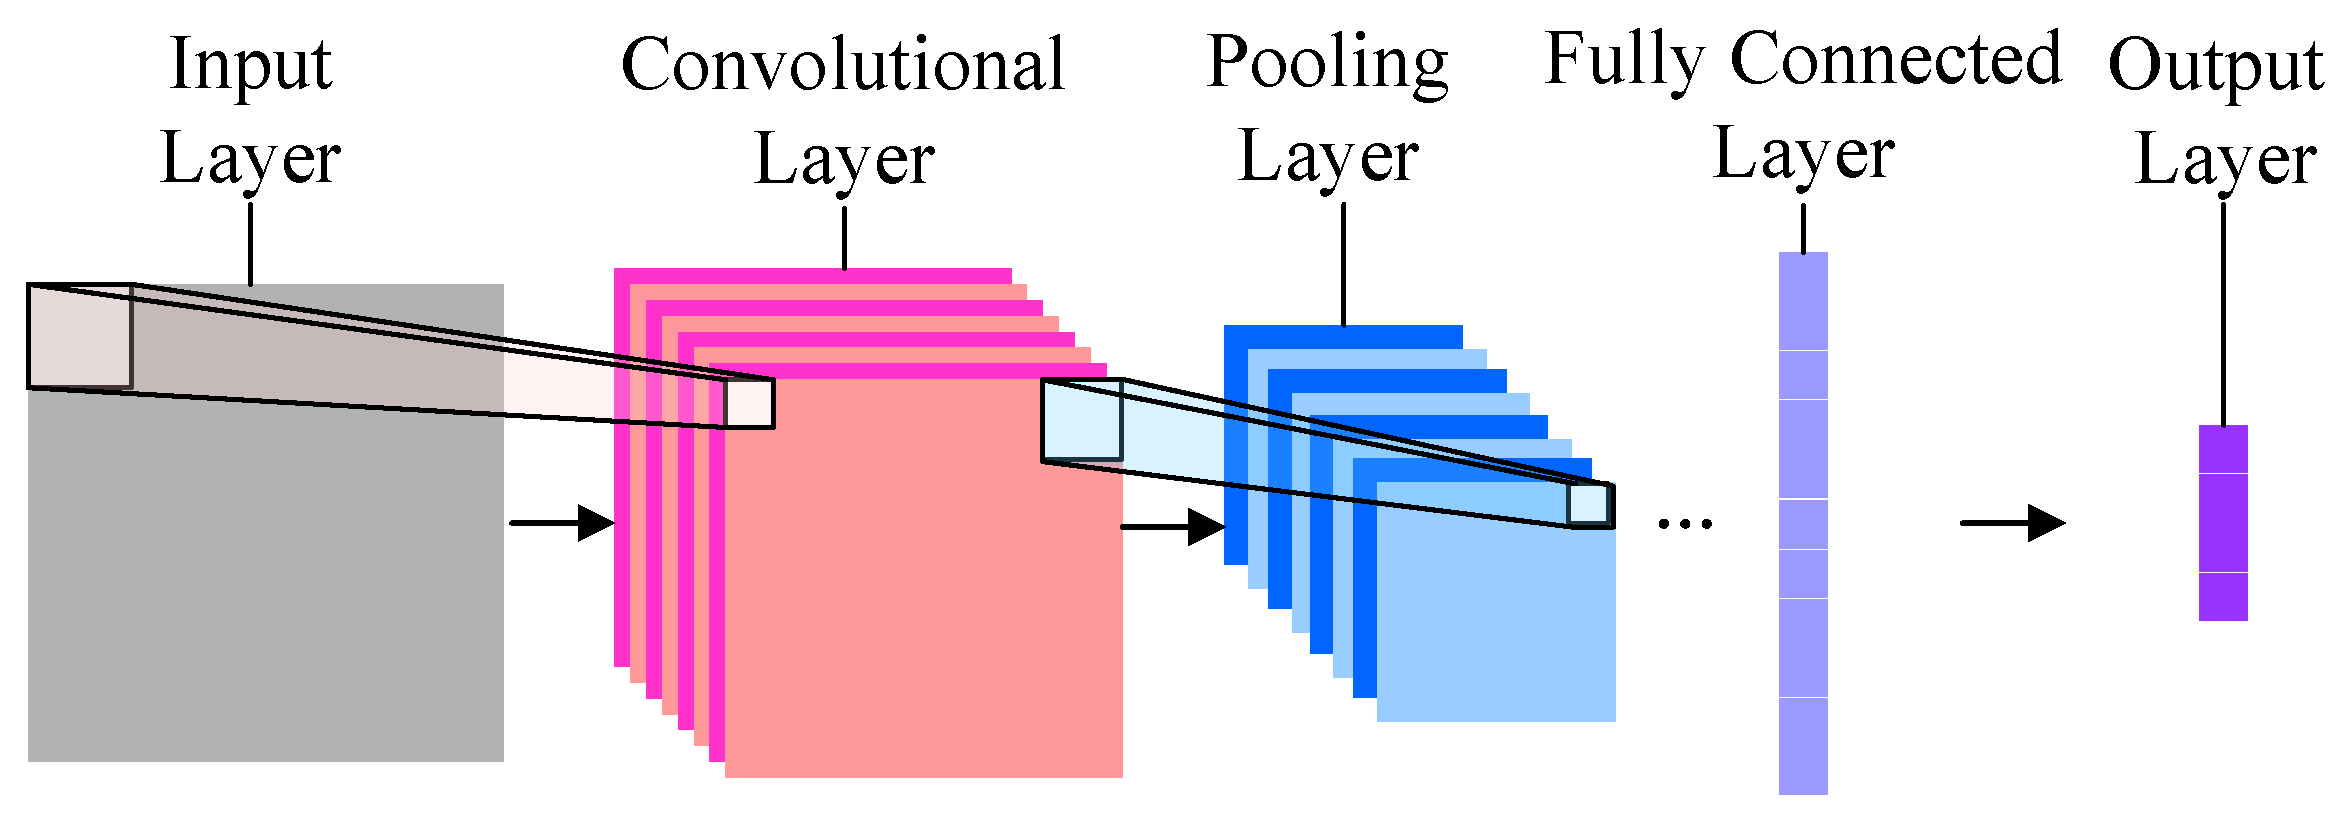
\includegraphics{convo.png}
\caption{CNN}
\end{figure}

    \paragraph{a) Convolution}\label{a-convolution}

ConvNets derive their name from the ``convolution'' operator. The
primary purpose of Convolution in case of a ConvNet is to extract
features from the input image. Convolution preserves the spatial
relationship between pixels by learning image features using small
squares of input data.

\paragraph{b) Pooling}\label{b-pooling}

Spatial Pooling (also called subsampling or downsampling) reduces the
dimensionality of each feature map but retains the most important
information. Spatial Pooling can be of different types: Max, Average,
Sum etc. In case of Max Pooling, we define a spatial neighborhood (for
example, a 2×2 window) and take the largest element from the rectified
feature map within that window. Instead of taking the largest element we
could also take the average (Average Pooling) or sum of all elements in
that window. In practice, Max Pooling has been shown to work better.

\paragraph{c) Flattening}\label{c-flattening}

Convert the 2D matrix to a column vector so that it can passed through
an artificial neural network

\paragraph{d) Full Connection}\label{d-full-connection}

The Fully Connected layer is a traditional Multi Layer Perceptron that
uses a softmax activation function in the output layer (other
classifiers like SVM can also be used, but will stick to softmax in this
post). The term ``Fully Connected'' implies that every neuron in the
previous layer is connected to every neuron on the next layer. The
output from the convolutional and pooling layers represent high-level
features of the input image. The purpose of the Fully Connected layer is
to use these features for classifying the input image into various
classes based on the training dataset.

    \subsection{4. Implementation of Speech Recognizer in
Tensorflow}\label{implementation-of-speech-recognizer-in-tensorflow}

    First we need to import the libararies required by the application

    \begin{Verbatim}[commandchars=\\\{\}]
{\color{incolor}In [{\color{incolor}8}]:} \PY{c+c1}{\PYZsh{}import required libraries}
        \PY{k+kn}{import} \PY{n+nn}{numpy} \PY{k}{as} \PY{n+nn}{np}                                    \PY{c+c1}{\PYZsh{}\PYZsh{}for numerical computations}
        \PY{k+kn}{import} \PY{n+nn}{librosa}                                        \PY{c+c1}{\PYZsh{}\PYZsh{}for converting to mfcc}
        \PY{k+kn}{import} \PY{n+nn}{os}                                             \PY{c+c1}{\PYZsh{}\PYZsh{}for file handling}
        \PY{k+kn}{from} \PY{n+nn}{keras}\PY{n+nn}{.}\PY{n+nn}{utils} \PY{k}{import} \PY{n}{to\PYZus{}categorical}                \PY{c+c1}{\PYZsh{}\PYZsh{}for one shot encoding}
        \PY{k+kn}{from} \PY{n+nn}{sklearn}\PY{n+nn}{.}\PY{n+nn}{model\PYZus{}selection} \PY{k}{import} \PY{n}{train\PYZus{}test\PYZus{}split}  \PY{c+c1}{\PYZsh{}\PYZsh{}split dataset into}
        \PY{k+kn}{import} \PY{n+nn}{tensorflow} \PY{k}{as} \PY{n+nn}{tf}                               \PY{c+c1}{\PYZsh{}\PYZsh{}tensorflow}
\end{Verbatim}


    \begin{Verbatim}[commandchars=\\\{\}]
Using TensorFlow backend.

    \end{Verbatim}

    \subsubsection{4.1. Dataset}\label{dataset}

    The dataset is located in folder named data, we set DATA\_PATH variable
to that folder.

    \begin{Verbatim}[commandchars=\\\{\}]
{\color{incolor}In [{\color{incolor}7}]:} \PY{n}{DATA\PYZus{}PATH} \PY{o}{=} \PY{l+s+s2}{\PYZdq{}}\PY{l+s+s2}{./data/}\PY{l+s+s2}{\PYZdq{}}
\end{Verbatim}


    The data consists of three classes, viz. bed, cat and happy.

    \begin{figure}
\centering

\includegraphics{download.png}
\caption{Data set}
\end{figure}

    Each folder contains approximately 1700 audio files. The name of the
folder is actually the label of those audio files. The task will be to
classify an audio between \textbf{bed, cat and happy} - these three
classes.

    \subsubsection{4.2. Preprocessing Audio
Files}\label{preprocessing-audio-files}

    We need to prepare a fixed size vector for each audio file and feed the
vector into the Convolutional Net.An \textbf{embedding} is a mapping
from discrete objects, such as words, to vectors of real numbers.

    \paragraph{Audio Embedding}\label{audio-embedding}

    \begin{figure}
\centering
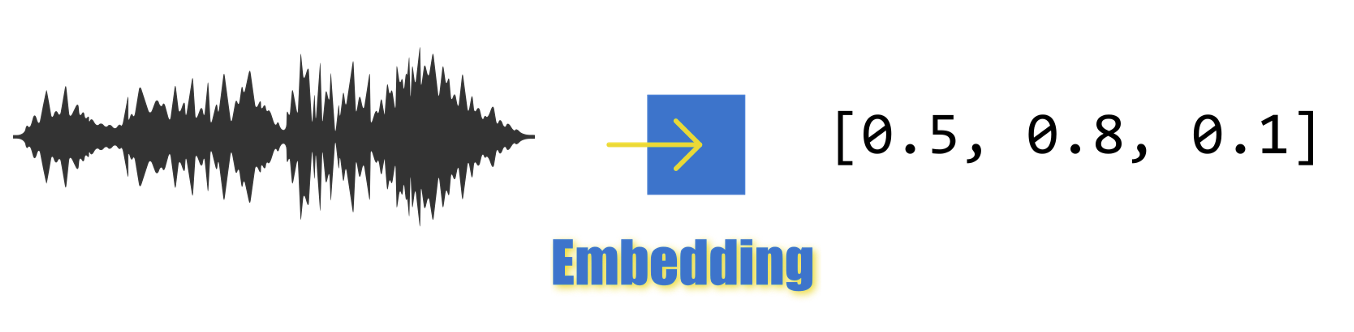
\includegraphics{Aembed.png}
\caption{Audion Embedding}
\end{figure}

In sound processing, the \textbf{mel-frequency cepstrum} (MFC) is a
representation of the short-term power spectrum of a sound, based on a
linear cosine transform of a log power spectrum on a nonlinear mel scale
of frequency.

    \paragraph{Steps}\label{steps}

\begin{enumerate}
\def\labelenumi{\arabic{enumi}.}
\item
  Read the audio file from DATA\_PATH.
\item
  Perform downsample operation.
\item
  Compute MFCC using librosa library.
\item
  MFCC vectors might vary in size for different audio input,To overcome
  this problem we need to pad the output vectors with zero.
\end{enumerate}

The function \textbf{wav2mfcc} performs the aforementioned steps.

    \begin{Verbatim}[commandchars=\\\{\}]
{\color{incolor}In [{\color{incolor}31}]:} \PY{k}{def} \PY{n+nf}{wav2mfcc}\PY{p}{(}\PY{n}{file\PYZus{}path}\PY{p}{,} \PY{n}{max\PYZus{}pad\PYZus{}len}\PY{o}{=}\PY{l+m+mi}{11}\PY{p}{)}\PY{p}{:}
             \PY{n}{wave}\PY{p}{,} \PY{n}{sr} \PY{o}{=} \PY{n}{librosa}\PY{o}{.}\PY{n}{load}\PY{p}{(}\PY{n}{file\PYZus{}path}\PY{p}{,} \PY{n}{mono}\PY{o}{=}\PY{k+kc}{True}\PY{p}{,} \PY{n}{sr}\PY{o}{=}\PY{k+kc}{None}\PY{p}{)}
             \PY{n}{wave} \PY{o}{=} \PY{n}{wave}\PY{p}{[}\PY{p}{:}\PY{p}{:}\PY{l+m+mi}{3}\PY{p}{]}
             \PY{n}{mfcc} \PY{o}{=} \PY{n}{librosa}\PY{o}{.}\PY{n}{feature}\PY{o}{.}\PY{n}{mfcc}\PY{p}{(}\PY{n}{wave}\PY{p}{,} \PY{n}{sr}\PY{o}{=}\PY{l+m+mi}{16000}\PY{p}{)}
             \PY{n}{pad\PYZus{}width} \PY{o}{=} \PY{n}{max\PYZus{}pad\PYZus{}len} \PY{o}{\PYZhy{}} \PY{n}{mfcc}\PY{o}{.}\PY{n}{shape}\PY{p}{[}\PY{l+m+mi}{1}\PY{p}{]}
             \PY{n}{mfcc} \PY{o}{=} \PY{n}{np}\PY{o}{.}\PY{n}{pad}\PY{p}{(}\PY{n}{mfcc}\PY{p}{,} \PY{n}{pad\PYZus{}width}\PY{o}{=}\PY{p}{(}\PY{p}{(}\PY{l+m+mi}{0}\PY{p}{,} \PY{l+m+mi}{0}\PY{p}{)}\PY{p}{,} \PY{p}{(}\PY{l+m+mi}{0}\PY{p}{,} \PY{n}{pad\PYZus{}width}\PY{p}{)}\PY{p}{)}\PY{p}{,} \PY{n}{mode}\PY{o}{=}\PY{l+s+s1}{\PYZsq{}}\PY{l+s+s1}{constant}\PY{l+s+s1}{\PYZsq{}}\PY{p}{)}
             \PY{k}{return} \PY{n}{mfcc}
\end{Verbatim}


    The function \textbf{get\_labels} gets the name of different categories
of data present in the dataset folder and encodes them

    \begin{Verbatim}[commandchars=\\\{\}]
{\color{incolor}In [{\color{incolor}9}]:} \PY{k}{def} \PY{n+nf}{get\PYZus{}labels}\PY{p}{(}\PY{n}{path}\PY{o}{=}\PY{n}{DATA\PYZus{}PATH}\PY{p}{)}\PY{p}{:}
            \PY{n}{labels} \PY{o}{=} \PY{n}{os}\PY{o}{.}\PY{n}{listdir}\PY{p}{(}\PY{n}{path}\PY{p}{)}
            \PY{n}{label\PYZus{}indices} \PY{o}{=} \PY{n}{np}\PY{o}{.}\PY{n}{arange}\PY{p}{(}\PY{l+m+mi}{0}\PY{p}{,} \PY{n+nb}{len}\PY{p}{(}\PY{n}{labels}\PY{p}{)}\PY{p}{)}
            \PY{k}{return} \PY{n}{labels}\PY{p}{,} \PY{n}{label\PYZus{}indices}\PY{p}{,} \PY{n}{to\PYZus{}categorical}\PY{p}{(}\PY{n}{label\PYZus{}indices}\PY{p}{)}
\end{Verbatim}


    In order to avoid the computation of mfcc again and again we store the
calculated data in a numpy array using the
\textbf{save\_data\_to\_array} function and can be resued for further
computations

    \begin{Verbatim}[commandchars=\\\{\}]
{\color{incolor}In [{\color{incolor}10}]:} \PY{k}{def} \PY{n+nf}{save\PYZus{}data\PYZus{}to\PYZus{}array}\PY{p}{(}\PY{n}{path}\PY{o}{=}\PY{n}{DATA\PYZus{}PATH}\PY{p}{,} \PY{n}{max\PYZus{}pad\PYZus{}len}\PY{o}{=}\PY{l+m+mi}{11}\PY{p}{)}\PY{p}{:}
             \PY{n}{labels}\PY{p}{,} \PY{n}{\PYZus{}}\PY{p}{,} \PY{n}{\PYZus{}} \PY{o}{=} \PY{n}{get\PYZus{}labels}\PY{p}{(}\PY{n}{path}\PY{p}{)}
         
             \PY{k}{for} \PY{n}{label} \PY{o+ow}{in} \PY{n}{labels}\PY{p}{:}
                 \PY{c+c1}{\PYZsh{} Init mfcc vectors}
                 \PY{n}{mfcc\PYZus{}vectors} \PY{o}{=} \PY{p}{[}\PY{p}{]}
         
                 \PY{n}{wavfiles} \PY{o}{=} \PY{p}{[}\PY{n}{path} \PY{o}{+} \PY{n}{label} \PY{o}{+} \PY{l+s+s1}{\PYZsq{}}\PY{l+s+s1}{/}\PY{l+s+s1}{\PYZsq{}} \PY{o}{+} \PY{n}{wavfile} 
                             \PY{k}{for} \PY{n}{wavfile} \PY{o+ow}{in} \PY{n}{os}\PY{o}{.}\PY{n}{listdir}\PY{p}{(}\PY{n}{path} \PY{o}{+} \PY{l+s+s1}{\PYZsq{}}\PY{l+s+s1}{/}\PY{l+s+s1}{\PYZsq{}} \PY{o}{+} \PY{n}{label}\PY{p}{)}\PY{p}{]}
                 \PY{k}{for} \PY{n}{wavfile} \PY{o+ow}{in} \PY{n}{wavfiles}\PY{p}{:}
                     \PY{n}{mfcc} \PY{o}{=} \PY{n}{wav2mfcc}\PY{p}{(}\PY{n}{wavfile}\PY{p}{,} \PY{n}{max\PYZus{}pad\PYZus{}len}\PY{o}{=}\PY{n}{max\PYZus{}pad\PYZus{}len}\PY{p}{)}
                     \PY{n}{mfcc\PYZus{}vectors}\PY{o}{.}\PY{n}{append}\PY{p}{(}\PY{n}{mfcc}\PY{p}{)}
                 \PY{n}{np}\PY{o}{.}\PY{n}{save}\PY{p}{(}\PY{n}{label} \PY{o}{+} \PY{l+s+s1}{\PYZsq{}}\PY{l+s+s1}{.npy}\PY{l+s+s1}{\PYZsq{}}\PY{p}{,} \PY{n}{mfcc\PYZus{}vectors}\PY{p}{)}
\end{Verbatim}


    The function \textbf{get\_train\_test} splits the entire dataset into
training set and test set. The training set contains 60 percent of the
data and test set contains 40 percent of the data.

    \begin{Verbatim}[commandchars=\\\{\}]
{\color{incolor}In [{\color{incolor}11}]:} \PY{k}{def} \PY{n+nf}{get\PYZus{}train\PYZus{}test}\PY{p}{(}\PY{n}{split\PYZus{}ratio}\PY{o}{=}\PY{l+m+mf}{0.6}\PY{p}{,} \PY{n}{random\PYZus{}state}\PY{o}{=}\PY{l+m+mi}{42}\PY{p}{)}\PY{p}{:}
             \PY{c+c1}{\PYZsh{} Get available labels}
             \PY{n}{labels}\PY{p}{,} \PY{n}{indices}\PY{p}{,} \PY{n}{\PYZus{}} \PY{o}{=} \PY{n}{get\PYZus{}labels}\PY{p}{(}\PY{n}{DATA\PYZus{}PATH}\PY{p}{)}
         
             \PY{c+c1}{\PYZsh{} Getting first arrays}
             \PY{n}{X} \PY{o}{=} \PY{n}{np}\PY{o}{.}\PY{n}{load}\PY{p}{(}\PY{n}{labels}\PY{p}{[}\PY{l+m+mi}{0}\PY{p}{]} \PY{o}{+} \PY{l+s+s1}{\PYZsq{}}\PY{l+s+s1}{.npy}\PY{l+s+s1}{\PYZsq{}}\PY{p}{)}
             \PY{n}{y} \PY{o}{=} \PY{n}{np}\PY{o}{.}\PY{n}{zeros}\PY{p}{(}\PY{n}{X}\PY{o}{.}\PY{n}{shape}\PY{p}{[}\PY{l+m+mi}{0}\PY{p}{]}\PY{p}{)}
         
             \PY{c+c1}{\PYZsh{} Append all of the dataset into one single array, same goes for y}
             \PY{k}{for} \PY{n}{i}\PY{p}{,} \PY{n}{label} \PY{o+ow}{in} \PY{n+nb}{enumerate}\PY{p}{(}\PY{n}{labels}\PY{p}{[}\PY{l+m+mi}{1}\PY{p}{:}\PY{p}{]}\PY{p}{)}\PY{p}{:}
                 \PY{n}{x} \PY{o}{=} \PY{n}{np}\PY{o}{.}\PY{n}{load}\PY{p}{(}\PY{n}{label} \PY{o}{+} \PY{l+s+s1}{\PYZsq{}}\PY{l+s+s1}{.npy}\PY{l+s+s1}{\PYZsq{}}\PY{p}{)}
                 \PY{n}{X} \PY{o}{=} \PY{n}{np}\PY{o}{.}\PY{n}{vstack}\PY{p}{(}\PY{p}{(}\PY{n}{X}\PY{p}{,} \PY{n}{x}\PY{p}{)}\PY{p}{)}
                 \PY{n}{y} \PY{o}{=} \PY{n}{np}\PY{o}{.}\PY{n}{append}\PY{p}{(}\PY{n}{y}\PY{p}{,} \PY{n}{np}\PY{o}{.}\PY{n}{full}\PY{p}{(}\PY{n}{x}\PY{o}{.}\PY{n}{shape}\PY{p}{[}\PY{l+m+mi}{0}\PY{p}{]}\PY{p}{,} \PY{n}{fill\PYZus{}value}\PY{o}{=} \PY{p}{(}\PY{n}{i} \PY{o}{+} \PY{l+m+mi}{1}\PY{p}{)}\PY{p}{)}\PY{p}{)}
         
             \PY{k}{assert} \PY{n}{X}\PY{o}{.}\PY{n}{shape}\PY{p}{[}\PY{l+m+mi}{0}\PY{p}{]} \PY{o}{==} \PY{n+nb}{len}\PY{p}{(}\PY{n}{y}\PY{p}{)}
         
             \PY{k}{return} \PY{n}{train\PYZus{}test\PYZus{}split}\PY{p}{(}\PY{n}{X}\PY{p}{,} \PY{n}{y}\PY{p}{,} \PY{n}{test\PYZus{}size}\PY{o}{=} \PY{p}{(}\PY{l+m+mi}{1} \PY{o}{\PYZhy{}} \PY{n}{split\PYZus{}ratio}\PY{p}{)}\PY{p}{,}
                                     \PY{n}{random\PYZus{}state}\PY{o}{=}\PY{n}{random\PYZus{}state}\PY{p}{,} \PY{n}{shuffle}\PY{o}{=}\PY{k+kc}{True}\PY{p}{)}
\end{Verbatim}


    Now we use get\_train\_test to split the dataset, We also use one hot
encoding to convert categorical data to appropriate formats which is
suitable for computation by the CNN

    \begin{Verbatim}[commandchars=\\\{\}]
{\color{incolor}In [{\color{incolor}19}]:} \PY{n}{X\PYZus{}train}\PY{p}{,} \PY{n}{X\PYZus{}test}\PY{p}{,} \PY{n}{y\PYZus{}train}\PY{p}{,} \PY{n}{y\PYZus{}test} \PY{o}{=} \PY{n}{get\PYZus{}train\PYZus{}test}\PY{p}{(}\PY{p}{)}
         \PY{n}{X\PYZus{}train} \PY{o}{=} \PY{n}{X\PYZus{}train}\PY{o}{.}\PY{n}{reshape}\PY{p}{(}\PY{n}{X\PYZus{}train}\PY{o}{.}\PY{n}{shape}\PY{p}{[}\PY{l+m+mi}{0}\PY{p}{]}\PY{p}{,} \PY{l+m+mi}{20}\PY{p}{,} \PY{l+m+mi}{11}\PY{p}{,} \PY{l+m+mi}{1}\PY{p}{)}
         \PY{n}{X\PYZus{}test} \PY{o}{=} \PY{n}{X\PYZus{}test}\PY{o}{.}\PY{n}{reshape}\PY{p}{(}\PY{n}{X\PYZus{}test}\PY{o}{.}\PY{n}{shape}\PY{p}{[}\PY{l+m+mi}{0}\PY{p}{]}\PY{p}{,} \PY{l+m+mi}{20}\PY{p}{,} \PY{l+m+mi}{11}\PY{p}{,} \PY{l+m+mi}{1}\PY{p}{)}
         \PY{n}{y\PYZus{}train\PYZus{}hot} \PY{o}{=} \PY{n}{to\PYZus{}categorical}\PY{p}{(}\PY{n}{y\PYZus{}train}\PY{p}{)}
         \PY{n}{y\PYZus{}test\PYZus{}hot} \PY{o}{=} \PY{n}{to\PYZus{}categorical}\PY{p}{(}\PY{n}{y\PYZus{}test}\PY{p}{)}
\end{Verbatim}


    \subsubsection{4.3 Building the Convolutional Neural
Network}\label{building-the-convolutional-neural-network}

The function \textbf{init\_weights} initializes the weights of the
network with some random values using tensorflow's random distribution
function.

    \paragraph{Initializing the weights of the
CNN}\label{initializing-the-weights-of-the-cnn}

    \begin{Verbatim}[commandchars=\\\{\}]
{\color{incolor}In [{\color{incolor}12}]:} \PY{k}{def} \PY{n+nf}{init\PYZus{}weights}\PY{p}{(}\PY{n}{shape}\PY{p}{)}\PY{p}{:}
             \PY{n}{init\PYZus{}random\PYZus{}dist} \PY{o}{=} \PY{n}{tf}\PY{o}{.}\PY{n}{truncated\PYZus{}normal}\PY{p}{(}\PY{n}{shape}\PY{p}{,} \PY{n}{stddev}\PY{o}{=}\PY{l+m+mf}{0.1}\PY{p}{)}
             \PY{k}{return} \PY{n}{tf}\PY{o}{.}\PY{n}{Variable}\PY{p}{(}\PY{n}{init\PYZus{}random\PYZus{}dist}\PY{p}{)}
\end{Verbatim}


    \paragraph{Initializing the bias of the
CNN}\label{initializing-the-bias-of-the-cnn}

This function \textbf{init\_bias} initializes the bias with some
constant value

    \begin{Verbatim}[commandchars=\\\{\}]
{\color{incolor}In [{\color{incolor}13}]:} \PY{k}{def} \PY{n+nf}{init\PYZus{}bias}\PY{p}{(}\PY{n}{shape}\PY{p}{)}\PY{p}{:}
             \PY{n}{init\PYZus{}bias\PYZus{}vals} \PY{o}{=} \PY{n}{tf}\PY{o}{.}\PY{n}{constant}\PY{p}{(}\PY{l+m+mf}{0.1}\PY{p}{,} \PY{n}{shape}\PY{o}{=}\PY{n}{shape}\PY{p}{)}
             \PY{k}{return} \PY{n}{tf}\PY{o}{.}\PY{n}{Variable}\PY{p}{(}\PY{n}{init\PYZus{}bias\PYZus{}vals}\PY{p}{)}
\end{Verbatim}


    \paragraph{Creating the Convolutional
layer}\label{creating-the-convolutional-layer}

The \textbf{conv2d} is a function that takes feature matrix x, and
weight matrix W as input and returns a 2d convolutional layer

    \begin{Verbatim}[commandchars=\\\{\}]
{\color{incolor}In [{\color{incolor}14}]:} \PY{k}{def} \PY{n+nf}{conv2d}\PY{p}{(}\PY{n}{x}\PY{p}{,} \PY{n}{W}\PY{p}{)}\PY{p}{:}
             \PY{k}{return} \PY{n}{tf}\PY{o}{.}\PY{n}{nn}\PY{o}{.}\PY{n}{conv2d}\PY{p}{(}\PY{n}{x}\PY{p}{,} \PY{n}{W}\PY{p}{,} \PY{n}{strides}\PY{o}{=}\PY{p}{[}\PY{l+m+mi}{1}\PY{p}{,} \PY{l+m+mi}{1}\PY{p}{,} \PY{l+m+mi}{1}\PY{p}{,} \PY{l+m+mi}{1}\PY{p}{]}\PY{p}{,} \PY{n}{padding}\PY{o}{=}\PY{l+s+s1}{\PYZsq{}}\PY{l+s+s1}{SAME}\PY{l+s+s1}{\PYZsq{}}\PY{p}{)}
\end{Verbatim}


    The 2x2 pooling layer is created by \textbf{max\_pool\_2by2}

    \begin{Verbatim}[commandchars=\\\{\}]
{\color{incolor}In [{\color{incolor}17}]:} \PY{k}{def} \PY{n+nf}{max\PYZus{}pool\PYZus{}2by2}\PY{p}{(}\PY{n}{x}\PY{p}{)}\PY{p}{:}
             \PY{k}{return} \PY{n}{tf}\PY{o}{.}\PY{n}{nn}\PY{o}{.}\PY{n}{max\PYZus{}pool}\PY{p}{(}\PY{n}{x}\PY{p}{,} \PY{n}{ksize}\PY{o}{=}\PY{p}{[}\PY{l+m+mi}{1}\PY{p}{,} \PY{l+m+mi}{2}\PY{p}{,} \PY{l+m+mi}{2}\PY{p}{,} \PY{l+m+mi}{1}\PY{p}{]}\PY{p}{,}
                                   \PY{n}{strides}\PY{o}{=}\PY{p}{[}\PY{l+m+mi}{1}\PY{p}{,} \PY{l+m+mi}{2}\PY{p}{,} \PY{l+m+mi}{2}\PY{p}{,} \PY{l+m+mi}{1}\PY{p}{]}\PY{p}{,} \PY{n}{padding}\PY{o}{=}\PY{l+s+s1}{\PYZsq{}}\PY{l+s+s1}{SAME}\PY{l+s+s1}{\PYZsq{}}\PY{p}{)}
\end{Verbatim}


    \textbf{convolutional\_layer} method uses conv2d to perform convolution
and passes it through a relu activation function

    \begin{Verbatim}[commandchars=\\\{\}]
{\color{incolor}In [{\color{incolor}16}]:} \PY{k}{def} \PY{n+nf}{convolutional\PYZus{}layer}\PY{p}{(}\PY{n}{input\PYZus{}x}\PY{p}{,} \PY{n}{shape}\PY{p}{)}\PY{p}{:}
             \PY{n}{W} \PY{o}{=} \PY{n}{init\PYZus{}weights}\PY{p}{(}\PY{n}{shape}\PY{p}{)}
             \PY{n}{b} \PY{o}{=} \PY{n}{init\PYZus{}bias}\PY{p}{(}\PY{p}{[}\PY{n}{shape}\PY{p}{[}\PY{l+m+mi}{3}\PY{p}{]}\PY{p}{]}\PY{p}{)}
             \PY{k}{return} \PY{n}{tf}\PY{o}{.}\PY{n}{nn}\PY{o}{.}\PY{n}{relu}\PY{p}{(}\PY{n}{conv2d}\PY{p}{(}\PY{n}{input\PYZus{}x}\PY{p}{,} \PY{n}{W}\PY{p}{)} \PY{o}{+} \PY{n}{b}\PY{p}{)}
\end{Verbatim}


    \textbf{normal\_full\_layer} creates a fully connected layer

    \begin{Verbatim}[commandchars=\\\{\}]
{\color{incolor}In [{\color{incolor}18}]:} \PY{k}{def} \PY{n+nf}{normal\PYZus{}full\PYZus{}layer}\PY{p}{(}\PY{n}{input\PYZus{}layer}\PY{p}{,} \PY{n}{size}\PY{p}{)}\PY{p}{:}
             \PY{n}{input\PYZus{}size} \PY{o}{=} \PY{n+nb}{int}\PY{p}{(}\PY{n}{input\PYZus{}layer}\PY{o}{.}\PY{n}{get\PYZus{}shape}\PY{p}{(}\PY{p}{)}\PY{p}{[}\PY{l+m+mi}{1}\PY{p}{]}\PY{p}{)}
             \PY{n}{W} \PY{o}{=} \PY{n}{init\PYZus{}weights}\PY{p}{(}\PY{p}{[}\PY{n}{input\PYZus{}size}\PY{p}{,} \PY{n}{size}\PY{p}{]}\PY{p}{)}
             \PY{n}{b} \PY{o}{=} \PY{n}{init\PYZus{}bias}\PY{p}{(}\PY{p}{[}\PY{n}{size}\PY{p}{]}\PY{p}{)}
             \PY{k}{return} \PY{n}{tf}\PY{o}{.}\PY{n}{matmul}\PY{p}{(}\PY{n}{input\PYZus{}layer}\PY{p}{,} \PY{n}{W}\PY{p}{)} \PY{o}{+} \PY{n}{b}
\end{Verbatim}


    The actual CNN is then created with the help of above helper functions.

    \begin{Verbatim}[commandchars=\\\{\}]
{\color{incolor}In [{\color{incolor}21}]:} \PY{c+c1}{\PYZsh{}\PYZsh{} using a 2x2 feature detector for convolution}
         \PY{c+c1}{\PYZsh{}\PYZsh{} There is a single input channel }
         \PY{c+c1}{\PYZsh{}\PYZsh{} And there will be 32 output features,}
         \PY{c+c1}{\PYZsh{}\PYZsh{} hence shape = [2, 2, 1, 32]}
         \PY{n}{convo\PYZus{}1} \PY{o}{=} \PY{n}{convolutional\PYZus{}layer}\PY{p}{(}\PY{n}{x}\PY{p}{,}\PY{n}{shape}\PY{o}{=}\PY{p}{[}\PY{l+m+mi}{2}\PY{p}{,}\PY{l+m+mi}{2}\PY{p}{,}\PY{l+m+mi}{1}\PY{p}{,}\PY{l+m+mi}{32}\PY{p}{]}\PY{p}{)}
         
         \PY{c+c1}{\PYZsh{}\PYZsh{} flattening the features extracted into an 1D array}
         \PY{c+c1}{\PYZsh{}\PYZsh{} The size of the array will be 20x11x32}
         \PY{n}{convo\PYZus{}2\PYZus{}flat} \PY{o}{=} \PY{n}{tf}\PY{o}{.}\PY{n}{reshape}\PY{p}{(}\PY{n}{convo\PYZus{}1}\PY{p}{,}\PY{p}{[}\PY{o}{\PYZhy{}}\PY{l+m+mi}{1}\PY{p}{,}\PY{l+m+mi}{20}\PY{o}{*}\PY{l+m+mi}{11}\PY{o}{*}\PY{l+m+mi}{32}\PY{p}{]}\PY{p}{)}
         
         \PY{c+c1}{\PYZsh{}\PYZsh{} creating a fully connected laer with 1024 neurons}
         \PY{c+c1}{\PYZsh{}\PYZsh{} It takes the 1D array conv\PYZus{}2\PYZus{}flat as input}
         \PY{n}{full\PYZus{}layer\PYZus{}one} \PY{o}{=} \PY{n}{tf}\PY{o}{.}\PY{n}{nn}\PY{o}{.}\PY{n}{relu}\PY{p}{(}\PY{n}{normal\PYZus{}full\PYZus{}layer}\PY{p}{(}\PY{n}{convo\PYZus{}2\PYZus{}flat}\PY{p}{,}\PY{l+m+mi}{1024}\PY{p}{)}\PY{p}{)}
         
         \PY{c+c1}{\PYZsh{}\PYZsh{} during training phase we need to randomly turn off }
         \PY{c+c1}{\PYZsh{}\PYZsh{} some neurons to find new paths in the network and }
         \PY{c+c1}{\PYZsh{}\PYZsh{} increase accuracy}
         \PY{n}{full\PYZus{}one\PYZus{}dropout} \PY{o}{=} \PY{n}{tf}\PY{o}{.}\PY{n}{nn}\PY{o}{.}\PY{n}{dropout}\PY{p}{(}\PY{n}{full\PYZus{}layer\PYZus{}one}\PY{p}{,}\PY{n}{keep\PYZus{}prob}\PY{o}{=}\PY{n}{hold\PYZus{}prob}\PY{p}{)}
         
         \PY{c+c1}{\PYZsh{}\PYZsh{} creating the final output layer with 3 neurons}
         \PY{c+c1}{\PYZsh{}\PYZsh{} to classify the audio into 3 categories}
         \PY{n}{y\PYZus{}pred} \PY{o}{=} \PY{n}{normal\PYZus{}full\PYZus{}layer}\PY{p}{(}\PY{n}{full\PYZus{}one\PYZus{}dropout}\PY{p}{,}\PY{l+m+mi}{3}\PY{p}{)}
\end{Verbatim}


    Defining the cost function of the network. In this case cross entropy is
being used. The objective of the CNN is to optimize the cost function.
We use Adam optimizer for our application. The learning rate \(\alpha\)
is 0.001

    \begin{Verbatim}[commandchars=\\\{\}]
{\color{incolor}In [{\color{incolor}23}]:} \PY{n}{cross\PYZus{}entropy} \PY{o}{=} \PY{n}{tf}\PY{o}{.}\PY{n}{reduce\PYZus{}mean}\PY{p}{(}
             \PY{n}{tf}\PY{o}{.}\PY{n}{nn}\PY{o}{.}\PY{n}{softmax\PYZus{}cross\PYZus{}entropy\PYZus{}with\PYZus{}logits\PYZus{}v2}\PY{p}{(}\PY{n}{labels}\PY{o}{=}\PY{n}{y\PYZus{}true}\PY{p}{,}
                                                        \PY{n}{logits}\PY{o}{=}\PY{n}{y\PYZus{}pred}\PY{p}{)}\PY{p}{)}
         \PY{n}{optimizer} \PY{o}{=} \PY{n}{tf}\PY{o}{.}\PY{n}{train}\PY{o}{.}\PY{n}{AdamOptimizer}\PY{p}{(}\PY{n}{learning\PYZus{}rate}\PY{o}{=}\PY{l+m+mf}{0.001}\PY{p}{)}
         \PY{n}{train} \PY{o}{=} \PY{n}{optimizer}\PY{o}{.}\PY{n}{minimize}\PY{p}{(}\PY{n}{cross\PYZus{}entropy}\PY{p}{)}
\end{Verbatim}


    \subsubsection{4.3 Training the CNN}\label{training-the-cnn}

    Tensorflow uses placeholders as special variables to feed data into Deep
Neural Networks. We define three placeholders as described below- 1. x:
input 2. y\_true: correct labels 3. hold\_prob: probability for dropout
layer

    \begin{Verbatim}[commandchars=\\\{\}]
{\color{incolor}In [{\color{incolor}20}]:} \PY{n}{x} \PY{o}{=} \PY{n}{tf}\PY{o}{.}\PY{n}{placeholder}\PY{p}{(}\PY{n}{tf}\PY{o}{.}\PY{n}{float32}\PY{p}{,}\PY{n}{shape}\PY{o}{=}\PY{p}{[}\PY{k+kc}{None}\PY{p}{,}\PY{l+m+mi}{20}\PY{p}{,}\PY{l+m+mi}{11}\PY{p}{,}\PY{l+m+mi}{1}\PY{p}{]}\PY{p}{)}
         \PY{n}{y\PYZus{}true} \PY{o}{=} \PY{n}{tf}\PY{o}{.}\PY{n}{placeholder}\PY{p}{(}\PY{n}{tf}\PY{o}{.}\PY{n}{float32}\PY{p}{,}\PY{n}{shape}\PY{o}{=}\PY{p}{[}\PY{k+kc}{None}\PY{p}{,}\PY{l+m+mi}{3}\PY{p}{]}\PY{p}{)}
         \PY{n}{hold\PYZus{}prob} \PY{o}{=} \PY{n}{tf}\PY{o}{.}\PY{n}{placeholder}\PY{p}{(}\PY{n}{tf}\PY{o}{.}\PY{n}{float32}\PY{p}{)}
\end{Verbatim}


    The graph nodes corresponding to the CNN are created by Tensorflow, and
the variables are initialized

    \begin{Verbatim}[commandchars=\\\{\}]
{\color{incolor}In [{\color{incolor}24}]:} \PY{n}{init} \PY{o}{=} \PY{n}{tf}\PY{o}{.}\PY{n}{global\PYZus{}variables\PYZus{}initializer}\PY{p}{(}\PY{p}{)}
\end{Verbatim}


    \textbf{saver} saves the model parameters and weights

    \begin{Verbatim}[commandchars=\\\{\}]
{\color{incolor}In [{\color{incolor}25}]:} \PY{n}{saver} \PY{o}{=} \PY{n}{tf}\PY{o}{.}\PY{n}{train}\PY{o}{.}\PY{n}{Saver}\PY{p}{(}\PY{p}{)}
\end{Verbatim}


    Now we create a Tensorflow session. The graph is initialized and the
session is run

    \begin{Verbatim}[commandchars=\\\{\}]
{\color{incolor}In [{\color{incolor}27}]:} \PY{k}{with} \PY{n}{tf}\PY{o}{.}\PY{n}{Session}\PY{p}{(}\PY{p}{)} \PY{k}{as} \PY{n}{sess}\PY{p}{:}
             \PY{n}{sess}\PY{o}{.}\PY{n}{run}\PY{p}{(}\PY{n}{init}\PY{p}{)}
             \PY{k}{for} \PY{n}{i} \PY{o+ow}{in} \PY{n+nb}{range}\PY{p}{(}\PY{l+m+mi}{250}\PY{p}{)}\PY{p}{:}
                 \PY{c+c1}{\PYZsh{}print(\PYZdq{}Training Epoch : \PYZdq{} + str(i))}
                 \PY{n}{sess}\PY{o}{.}\PY{n}{run}\PY{p}{(}\PY{n}{train}\PY{p}{,} \PY{n}{feed\PYZus{}dict}\PY{o}{=}\PY{p}{\PYZob{}}\PY{n}{x}\PY{p}{:} \PY{n}{X\PYZus{}train}\PY{p}{,}
                                            \PY{n}{y\PYZus{}true}\PY{p}{:} \PY{n}{y\PYZus{}train\PYZus{}hot}\PY{p}{,} \PY{n}{hold\PYZus{}prob}\PY{p}{:} \PY{l+m+mf}{0.5}\PY{p}{\PYZcb{}}\PY{p}{)}
                 
                 \PY{c+c1}{\PYZsh{} PRINT OUT A MESSAGE EVERY 100 STEPS}
                 \PY{k}{if} \PY{n}{i}\PY{o}{\PYZpc{}}\PY{k}{100} == 0:
                     
                     \PY{n+nb}{print}\PY{p}{(}\PY{l+s+s1}{\PYZsq{}}\PY{l+s+s1}{Currently on step }\PY{l+s+si}{\PYZob{}\PYZcb{}}\PY{l+s+s1}{\PYZsq{}}\PY{o}{.}\PY{n}{format}\PY{p}{(}\PY{n}{i}\PY{p}{)}\PY{p}{)}
                     \PY{n+nb}{print}\PY{p}{(}\PY{l+s+s1}{\PYZsq{}}\PY{l+s+s1}{Accuracy is:}\PY{l+s+s1}{\PYZsq{}}\PY{p}{)}
                     \PY{c+c1}{\PYZsh{} Test the Train Model}
                     \PY{n}{matches} \PY{o}{=} \PY{n}{tf}\PY{o}{.}\PY{n}{equal}\PY{p}{(}\PY{n}{tf}\PY{o}{.}\PY{n}{argmax}\PY{p}{(}\PY{n}{y\PYZus{}pred}\PY{p}{,}\PY{l+m+mi}{1}\PY{p}{)}\PY{p}{,}\PY{n}{tf}\PY{o}{.}\PY{n}{argmax}\PY{p}{(}\PY{n}{y\PYZus{}true}\PY{p}{,}\PY{l+m+mi}{1}\PY{p}{)}\PY{p}{)}
         
                     \PY{n}{acc} \PY{o}{=} \PY{n}{tf}\PY{o}{.}\PY{n}{reduce\PYZus{}mean}\PY{p}{(}\PY{n}{tf}\PY{o}{.}\PY{n}{cast}\PY{p}{(}\PY{n}{matches}\PY{p}{,}\PY{n}{tf}\PY{o}{.}\PY{n}{float32}\PY{p}{)}\PY{p}{)}
                     \PY{n+nb}{print}\PY{p}{(}\PY{n}{sess}\PY{o}{.}\PY{n}{run}\PY{p}{(}\PY{n}{acc}\PY{p}{,}\PY{n}{feed\PYZus{}dict}\PY{o}{=}\PY{p}{\PYZob{}}\PY{n}{x}\PY{p}{:}\PY{n}{X\PYZus{}test}\PY{p}{,}
                                                   \PY{n}{y\PYZus{}true}\PY{p}{:}\PY{n}{y\PYZus{}test\PYZus{}hot}\PY{p}{,}\PY{n}{hold\PYZus{}prob}\PY{p}{:}\PY{l+m+mf}{1.0}\PY{p}{\PYZcb{}}\PY{p}{)}\PY{p}{)}
             
             \PY{n}{saver}\PY{o}{.}\PY{n}{save}\PY{p}{(}\PY{n}{sess}\PY{p}{,}\PY{l+s+s1}{\PYZsq{}}\PY{l+s+s1}{models/cnn\PYZus{}model.ckpt}\PY{l+s+s1}{\PYZsq{}}\PY{p}{)}
\end{Verbatim}


    \begin{Verbatim}[commandchars=\\\{\}]
Currently on step 0
Accuracy is:
0.3261079
Currently on step 100
Accuracy is:
0.9238921
Currently on step 200
Accuracy is:
0.9349711

    \end{Verbatim}

    \begin{Verbatim}[commandchars=\\\{\}]
{\color{incolor}In [{\color{incolor}28}]:} \PY{c+c1}{\PYZsh{}Prediction on a new voice}
         \PY{k+kn}{from} \PY{n+nn}{tkinter} \PY{k}{import} \PY{n}{filedialog}
         \PY{k+kn}{from} \PY{n+nn}{tkinter} \PY{k}{import} \PY{n}{Tk}\PY{p}{,}\PY{n}{Label}\PY{p}{,}\PY{n}{Button}\PY{p}{,}\PY{n}{Canvas}
\end{Verbatim}


    \begin{Verbatim}[commandchars=\\\{\}]
{\color{incolor}In [{\color{incolor}29}]:} \PY{k}{def} \PY{n+nf}{browse\PYZus{}button}\PY{p}{(}\PY{p}{)}\PY{p}{:}
             \PY{c+c1}{\PYZsh{} Allow user to select a directory and store it in global var}
             \PY{c+c1}{\PYZsh{} called folder\PYZus{}path}
             \PY{k}{global} \PY{n}{folder\PYZus{}path}
             \PY{k}{global} \PY{n}{path}
             \PY{n}{filename} \PY{o}{=} \PY{n}{filedialog}\PY{o}{.}\PY{n}{askopenfile}\PY{p}{(}\PY{p}{)}
             \PY{n}{sample} \PY{o}{=} \PY{n}{wav2mfcc}\PY{p}{(}\PY{n}{filename}\PY{o}{.}\PY{n}{name}\PY{p}{)}
             \PY{n+nb}{print}\PY{p}{(}\PY{n}{filename}\PY{o}{.}\PY{n}{name}\PY{p}{)}
             \PY{n}{path} \PY{o}{=} \PY{l+s+s2}{\PYZdq{}}\PY{l+s+s2}{aplay }\PY{l+s+s2}{\PYZdq{}} \PY{o}{+} \PY{n}{filename}\PY{o}{.}\PY{n}{name}\PY{p}{[}\PY{l+m+mi}{50}\PY{p}{:}\PY{p}{]}
             \PY{n}{sample\PYZus{}reshaped} \PY{o}{=} \PY{n}{sample}\PY{o}{.}\PY{n}{reshape}\PY{p}{(}\PY{l+m+mi}{1}\PY{p}{,} \PY{l+m+mi}{20}\PY{p}{,} \PY{l+m+mi}{11}\PY{p}{,} \PY{l+m+mi}{1}\PY{p}{)}
             \PY{n}{labels} \PY{o}{=} \PY{p}{[}\PY{l+s+s2}{\PYZdq{}}\PY{l+s+s2}{happy}\PY{l+s+s2}{\PYZdq{}}\PY{p}{,} \PY{l+s+s2}{\PYZdq{}}\PY{l+s+s2}{cat}\PY{l+s+s2}{\PYZdq{}}\PY{p}{,} \PY{l+s+s2}{\PYZdq{}}\PY{l+s+s2}{bed}\PY{l+s+s2}{\PYZdq{}}\PY{p}{]}
             \PY{k}{with} \PY{n}{tf}\PY{o}{.}\PY{n}{Session}\PY{p}{(}\PY{p}{)} \PY{k}{as} \PY{n}{sess} \PY{p}{:}
                 \PY{n}{saver}\PY{o}{.}\PY{n}{restore}\PY{p}{(}\PY{n}{sess}\PY{p}{,}\PY{l+s+s1}{\PYZsq{}}\PY{l+s+s1}{models/cnn\PYZus{}model.ckpt}\PY{l+s+s1}{\PYZsq{}}\PY{p}{)}
                 \PY{n}{predict} \PY{o}{=} \PY{n}{tf}\PY{o}{.}\PY{n}{argmax}\PY{p}{(}\PY{n}{y\PYZus{}pred}\PY{p}{,}\PY{l+m+mi}{1}\PY{p}{)}
                 \PY{n}{pred} \PY{o}{=} \PY{n}{sess}\PY{o}{.}\PY{n}{run}\PY{p}{(}\PY{n}{predict}\PY{p}{,}
                                 \PY{n}{feed\PYZus{}dict}\PY{o}{=}\PY{p}{\PYZob{}}\PY{n}{x}\PY{p}{:}\PY{n}{sample\PYZus{}reshaped}\PY{p}{,}
                                            \PY{n}{y\PYZus{}true}\PY{p}{:} \PY{n}{y\PYZus{}train\PYZus{}hot}\PY{p}{,} \PY{n}{hold\PYZus{}prob}\PY{p}{:} \PY{l+m+mf}{1.0}\PY{p}{\PYZcb{}}\PY{p}{)}
                 \PY{n}{ans} \PY{o}{=} \PY{n}{labels}\PY{p}{[}\PY{n}{pred}\PY{p}{[}\PY{l+m+mi}{0}\PY{p}{]}\PY{p}{]}
                 \PY{n}{canvas}\PY{o}{.}\PY{n}{create\PYZus{}text}\PY{p}{(}\PY{l+m+mi}{350}\PY{p}{,} \PY{l+m+mi}{25}\PY{p}{,} 
                         \PY{n}{text} \PY{o}{=} \PY{l+s+s2}{\PYZdq{}}\PY{l+s+s2}{The detected word is : }\PY{l+s+s2}{\PYZdq{}} \PY{o}{+} \PY{n}{ans}\PY{p}{,} \PY{n}{font}\PY{o}{=}\PY{p}{(}\PY{l+s+s2}{\PYZdq{}}\PY{l+s+s2}{Purisa}\PY{l+s+s2}{\PYZdq{}}\PY{p}{,} \PY{l+m+mi}{25}\PY{p}{)}\PY{p}{)} 
\end{Verbatim}


    \begin{Verbatim}[commandchars=\\\{\}]
{\color{incolor}In [{\color{incolor}32}]:} \PY{n}{root} \PY{o}{=} \PY{n}{Tk}\PY{p}{(}\PY{p}{)}
         \PY{n}{root}\PY{o}{.}\PY{n}{title}\PY{p}{(}\PY{l+s+s2}{\PYZdq{}}\PY{l+s+s2}{Welcome to voice predictor}\PY{l+s+s2}{\PYZdq{}}\PY{p}{)} 
         \PY{n}{root}\PY{o}{.}\PY{n}{geometry}\PY{p}{(}\PY{l+s+s1}{\PYZsq{}}\PY{l+s+s1}{800x600}\PY{l+s+s1}{\PYZsq{}}\PY{p}{)}
         \PY{n}{button2} \PY{o}{=} \PY{n}{Button}\PY{p}{(}\PY{n}{text}\PY{o}{=}\PY{l+s+s2}{\PYZdq{}}\PY{l+s+s2}{Browse Audio File}\PY{l+s+s2}{\PYZdq{}}\PY{p}{,}
                          \PY{n}{command}\PY{o}{=}\PY{n}{browse\PYZus{}button}\PY{p}{,} \PY{n}{height} \PY{o}{=} \PY{l+m+mi}{1}\PY{p}{,}
                          \PY{n}{width} \PY{o}{=} \PY{l+m+mi}{20}\PY{p}{,}\PY{n}{font}\PY{o}{=}\PY{p}{(}\PY{l+s+s2}{\PYZdq{}}\PY{l+s+s2}{Ariel}\PY{l+s+s2}{\PYZdq{}}\PY{p}{,} \PY{l+m+mi}{15}\PY{p}{)}\PY{p}{)}
         \PY{n}{button2}\PY{o}{.}\PY{n}{pack}\PY{p}{(}\PY{p}{)}
         \PY{n}{canvas} \PY{o}{=} \PY{n}{Canvas}\PY{p}{(}\PY{n}{width}\PY{o}{=}\PY{l+m+mi}{700}\PY{p}{,} \PY{n}{height}\PY{o}{=}\PY{l+m+mi}{50}\PY{p}{,} \PY{n}{bg}\PY{o}{=}\PY{l+s+s1}{\PYZsq{}}\PY{l+s+s1}{green}\PY{l+s+s1}{\PYZsq{}}\PY{p}{)}
         \PY{n}{canvas}\PY{o}{.}\PY{n}{pack}\PY{p}{(}\PY{p}{)}
         \PY{n}{play} \PY{o}{=} \PY{k}{lambda} \PY{p}{:} \PY{n}{os}\PY{o}{.}\PY{n}{system}\PY{p}{(}\PY{n}{path}\PY{p}{)}
         \PY{n}{button} \PY{o}{=} \PY{n}{Button}\PY{p}{(}\PY{n}{root}\PY{p}{,} \PY{n}{text} \PY{o}{=} \PY{l+s+s1}{\PYZsq{}}\PY{l+s+s1}{Play Word Sound}\PY{l+s+s1}{\PYZsq{}}\PY{p}{,}
                         \PY{n}{command} \PY{o}{=} \PY{n}{play}\PY{p}{,} \PY{n}{height} \PY{o}{=} \PY{l+m+mi}{1}\PY{p}{,} \PY{n}{width} \PY{o}{=} \PY{l+m+mi}{20}\PY{p}{,}\PY{n}{font}\PY{o}{=}\PY{p}{(}\PY{l+s+s2}{\PYZdq{}}\PY{l+s+s2}{Purisa}\PY{l+s+s2}{\PYZdq{}}\PY{p}{,} \PY{l+m+mi}{15}\PY{p}{)}\PY{p}{)}
         \PY{n}{button}\PY{o}{.}\PY{n}{pack}\PY{p}{(}\PY{p}{)}
         \PY{n}{root}\PY{o}{.}\PY{n}{mainloop}\PY{p}{(}\PY{p}{)}
\end{Verbatim}


    \begin{Verbatim}[commandchars=\\\{\}]
/home/kemanth/Machine Learning/Speech Recognition/data/cat/0ab3b47d\_nohash\_0.wav
INFO:tensorflow:Restoring parameters from models/cnn\_model.ckpt

    \end{Verbatim}


    % Add a bibliography block to the postdoc
    
    
    
    \end{document}
